\documentclass[11pt]{article}
\usepackage{mathtools}
\usepackage{mdframed}
\usepackage{fullpage}
\usepackage{amsfonts}
\usepackage{tikz}
\usepackage{fancyhdr}
\usepackage{lastpage}
\usepackage{listings}
\lstset{language=C,
                basicstyle=\ttfamily,
                keywordstyle=\color{blue}\ttfamily,
                stringstyle=\color{red}\ttfamily,
                commentstyle=\color{green}\ttfamily,
                morecomment=[l][\color{magenta}]{\#}
}
\usetikzlibrary{automata, positioning}

%edit this for each class
\newcommand\name{John Collin Vincent}
\newcommand\classname{}
\newcommand\assignment{}


\newcounter{excounter}
\setcounter{excounter}{1}
\newcommand\ques[2]{\vskip 1em  \noindent\textbf{\arabic{excounter}\addtocounter{excounter}{1}.} \emph{#1} \noindent#2}
\newenvironment{question}{\ques{}\begin{quote}}{\end{quote}}
\newenvironment{subquestion}[1]{#1) \begin{quote}}{\end{quote}}

\pagestyle{fancy}
\rfoot{\name, page \thepage/\pageref{LastPage}}
\cfoot{}
\rhead{}
\lhead{}
\renewcommand{\headrulewidth}{0pt}
\renewcommand{\footrulewidth}{0pt}
\DeclarePairedDelimiter\ceil{\lceil}{\rceil}
\DeclarePairedDelimiter\floor{\lfloor}{\rfloor}


\begin{document}


  {\bf \classname \hspace{1cm} \assignment\hfill \name}
  \vskip 2em
    
    \begin{question}
        \begin{verbatim}
            -?[0-9]*(?:0|5)
        \end{verbatim}
    \end{question}

    \begin{question}
        \center
        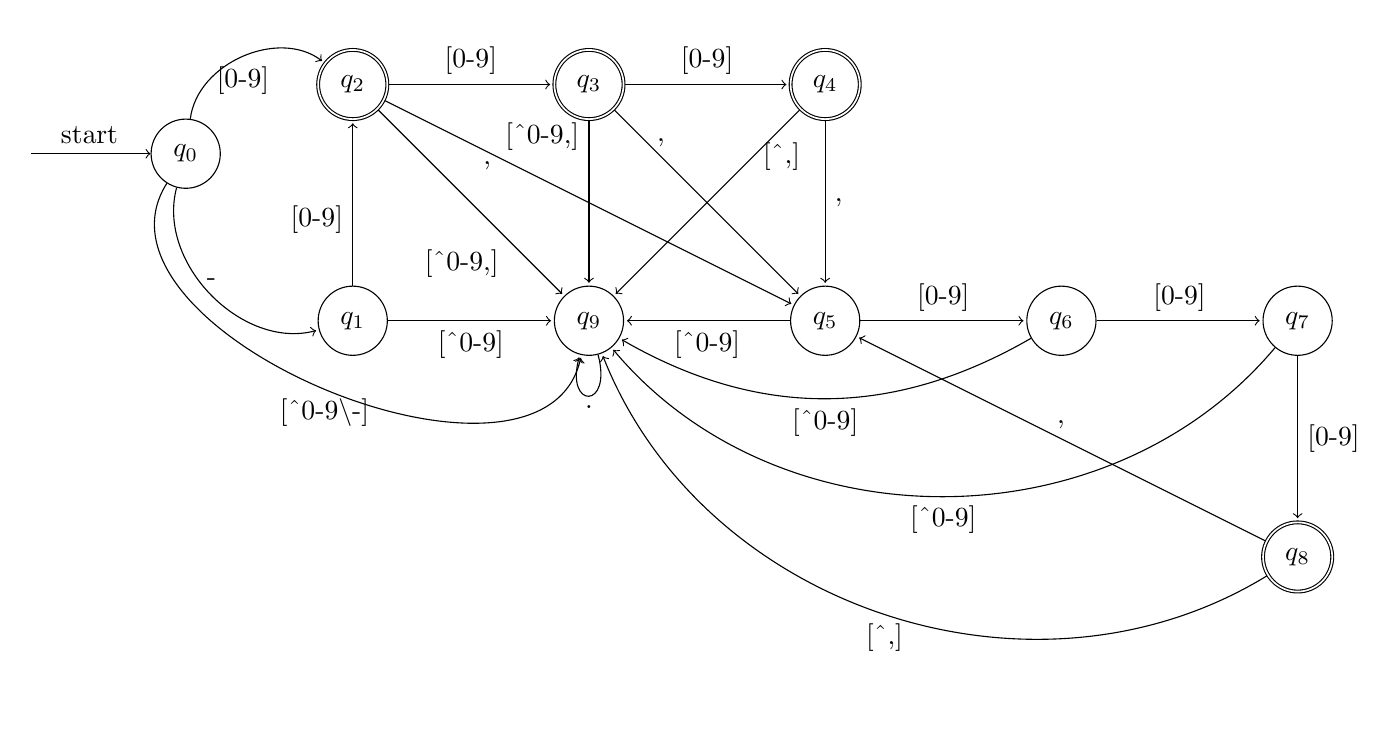
\begin{tikzpicture}[shorten >=1pt,node distance=3cm,on grid,auto]
            \node[state] (q_0) {$q_0$};
            \node[state] (q_1) [below right=of q_0] {$q_1$};
            \node[state, accepting] (q_2) [above=of q_1] {$q_2$};
            \node[state, accepting] (q_3) [right=of q_2] {$q_3$};
            \node[state, accepting] (q_4) [right=of q_3] {$q_4$};
            \node[state] (q_5) [below=of q_4] {$q_5$};
            \node[state] (q_6) [right=of q_5] {$q_6$};
            \node[state] (q_7) [right=of q_6] {$q_7$};
            \node[state, accepting] (q_8) [below=of q_7] {$q_8$};
            \node[state] (q_9) [below=of q_3] {$q_9$};
            \draw[<-] (q_0) -- node[above] {start} ++(-2cm, 0);
            \path[->]
                (q_0) edge [bend right=60] node [above] {-} (q_1)
                edge [bend left=60] node [below] {[0-9]} (q_2)
                edge [bend right=100] node [below] {[\string^0-9\textbackslash-]} (q_9);
            \path[->]
                (q_1) edge [ pos=.4] node [left] {[0-9]} (q_2)
                edge node [below] {[\string^0-9]} (q_9);
            \path[->]
                (q_2) edge node [above] {[0-9]} (q_3)
                edge [pos=.7] node [below left] {[\string^0-9,]} (q_9)
                edge [pos=.25] node [below] {,} (q_5);
            \path[->]
                (q_3) edge node [above] {[0-9]} (q_4)
                edge [pos=.1] node [left] {[\string^0-9,]} (q_9)
                edge [pos=.25] node [above] {,} (q_5);
            \path[->]
                (q_4) edge [pos=.25] node [right] {[\string^,]} (q_9)
                edge node [right] {,} (q_5);
            \path[->]
                (q_5) edge node [above] {[0-9]} (q_6)
                edge node [below] {[\string^0-9]} (q_9);
            \path[->]
                (q_6) edge node [above] {[0-9]} (q_7)
                edge [bend left=30] node [below] {[\string^0-9]} (q_9);
            \path[->]
                (q_7) edge node [right] {[0-9]} (q_8)
                edge [bend left=50] node [below] {[\string^0-9]} (q_9);
            \path[->]
                (q_8) edge node [above] {,} (q_5)
                edge [bend left=50] node [below] {[\string^,]} (q_9);
            \path[->]
                (q_9) edge [loop below] node {.} (q_9);
        \end{tikzpicture}
    \end{question}

    \clearpage

    \ques{}
    \begin{lstlisting}
    char* skipSpaces(char* buffer)
    {
        int i = 0;
        /*loop until target is found*/
        while(1)
        {
            /*handle 1 character at a time*/
            switch(buffer[i])
            {
                /*if its a basic space then skip it*/
                case '\t':
                case '\n':
                case ' ':
                    i++;
                    break;
                /*if it might be a c style investigate more*/
                case '/':
                    /*if it is a c style skip whole comment*/
                    if(buffer[i+1] == '*')
                    {
                        /*advance past the two opening and potentially 
                        2 closing characters*/
                        i+=4;
                        /*while the string has not been terminated or the end 
                        of the comment has not been reached just advance 
                        the pointer*/
                        while(buffer[i] != '\0' && 
                            (buffer[i-2] != '*' || buffer[i-1] != '/'))
                        {
                            i++;
                        }
                    }/*if not cstyle return */
                    else
                        return buffer+i;
                    break;
                default:
                    /* if its not one of the spaces then return*/
                    return buffer + i;
            }
        }
    }   
    \end{lstlisting}

\end{document}
